\documentclass[11pt]{article} 
\usepackage[utf8]{inputenc} 


\usepackage{geometry} 
\geometry{a4paper} 

\usepackage{graphicx} 
\usepackage{booktabs} 
\usepackage{array}
\usepackage{paralist} 
\usepackage{verbatim}
\usepackage{subfig}
\usepackage{amssymb}
\usepackage{amsmath}
\usepackage{titlesec}
\usepackage{tikz}

\usetikzlibrary{trees,arrows}

\setcounter{secnumdepth}{4}


\usepackage{fancyhdr} 
\pagestyle{fancy} 
\renewcommand{\headrulewidth}{0pt} 
\lhead{}\chead{}\rhead{}
\lfoot{}\cfoot{\thepage}\rfoot{}


\usepackage{sectsty}
\allsectionsfont{\sffamily\mdseries\upshape} 


\usepackage[nottoc,notlof,notlot]{tocbibind}
\usepackage[titles,subfigure]{tocloft} 
\renewcommand{\cftsecfont}{\rmfamily\mdseries\upshape}
\renewcommand{\cftsecpagefont}{\rmfamily\mdseries\upshape} 

\renewcommand{\P}{\mathbf{P}}
\newcommand{\NP}{\mathbf{NP}}
\newcommand{\RP}{\mathbf{RP}}
\newcommand{\CoRP}{\textbf{Co-}\mathbf{RP}}
\newcommand{\PPT}{\mathbf{PPT}}
\newcommand{\BPP}{\mathbf{BPP}}

\newcommand{\N}{\mathbb{N}}

\newcommand{\mcH}{\mathcal{H}}
\newcommand{\mcU}{\mathcal{U}}



\title{CS 183 Notes}
\author{Stephen Kelman\\ Rafi Ostrovsky, Eli Jaffe}


\begin{document}




\section{Lecture 6: Digital Signatures}

What we are looking for in this lecture is some way for us to sign documents,confirming our identity and our consent/acknowledgment of something, without someone being able to forge our signature.\smallskip

The first (obvious) thing to notice is that computers can copy bits by reading them in and spitting them out, so the signature has to change in some way. And, we don't want signatures to be able to moved from document to document by an adversary (think about the chaos this could cause!). So, we are going to solve both of these by having the signature depend on the document we are signing.

Formally, we define a ``\textbf{signature scheme}" as a protocol consisting of \(3\) \(\PPT\) algorithms:
\begin{enumerate}
\item \textbf{Keygen} takes in a security parameter \(k\) and some randomness. In return, it produces a \emph{public key} \(PK\), which is to be shared with everyone, and a \emph{signature key} \(SK\), or private key, which is to be shared with no one other than the signer.
\item \textbf{Sign} takes a document \(D\), both keys \(PK\) and \(SK\), and some randomness. In return, it produces a signature \(\sigma(D)\), which corresponds directly to the document being signed.
\item \textbf{Verify} takes the publickey \(PK\), a document \(D\), and a signature \(\sigma(D)\). In return, it returns a decision (accept/reject), accepting i.f.f. \(\sigma(D)\) is the proper signature of the document.
\end{enumerate}
Additionally, these \(3\) functions must together satisfy the following criteria:
\begin{enumerate}
\item \textbf{Correctness}: if Keygen and Sign are run properly, then Verify will accept all documents and their corresponding proper signatures.
\item \textbf{(Existential) Unforgeability}: No \(\PPT\) adversary can win at the following game except with negligible probability:
\end{enumerate}
This game is played between a challenger \(C\) who will sign documents, and an adversary \(A\) who will attempt to forge \(C\)'s signature on some new document.
\begin{enumerate}
\item [0.] \(C\) runs Keygen and sends \(PK\) to \(A\)
\item For some polynomial number of trials: \(A\) sends a document \(D\) to be signed, and \(C\) sends back the true proper signature \(\sigma(D)\)
\item \(A\) wins if it can, after polynomially many trials, send a document \(D^*\) and a signature \(\sigma(D^*)\) such that:
\begin{enumerate}
\item \(D^*\) was not sent in any of the trials
\item Verify(\(PK\), \(D^*\), \(\sigma(D^*)\)) accepts
\end{enumerate}
\end{enumerate}

We add two notes to this. \smallskip 

First, this game raises the concern that we should not be able to generate a valid signature of \(\sigma(D_1||D_2)\) from valid signatures of \(D_1\) and \(D_2\), or else any adversary could simply ask for \(D_1=0\) and \(D_2=1\) and then properly sign any document.\smallskip

Second, we add the note that a ``\textbf{strong signature scheme}" is one for which an adversary cannot come up with a different legal signature for \(D\), given \(D\) and some valid signature \(\sigma(D)\). (Note that this is possible, since the signing scheme involves randomness at every step.)

\subsection{Trapdoor Permutations}
We have seen 1WP's, but now we consider a different type of permutation which is hard to invert: a ``\emph{trapdoor permutation}". The idea is that for an arbitrary \(\PPT\) adversary, the trapdoor permutation should be as hard to invert as  a 1WP. But if an adversary is given access to some trapdoor \(t\), then it would be trivial for them to invert the permutation.\medskip

But as always, we are considering all adversaries, so we have to account for the adversary with the trapdoor hard-coded into it. In fact, since we are considering all polytime adversaries, we have to consider any adversary with polynomially many of these trapdoors for different permutations hard-coded into it. \smallskip

The solution to this issue is to use an exponentially large family of trapdoor permutations, rather than a single one. Then, each time we need to do something with a trapdoor permutation, we randomly sample from the family. Then, the probability that any given adversary knows the trapdoor for any particular use of our family is negigible, as desired.

\subsubsection{A (Faulty) Idea}
Now, with a family of trapdoor permutations in hand, we might try the following signature scheme:
\begin{enumerate}
\item Keygen picks a trapdoor permutation \(f\) from the family, and assigns \(PK\) to be \(f\) and \(SK\) to be the trapdoor \(t\)
\item Sign simply uses the trapdoor to compute \(f^{-1}\) of the document.
\item Verify can compute \(f\), given the signature, and checks that it matches the document
\end{enumerate}

The problem with this is very subtle and lies in something that we did not explicitly state here, as we defined the ``hardness" of inverting trapdoor permutations based on inverting 1WP's. The trouble is that an important aspect of the hardness of 1WP's, and thus trapdoor permutations, is that we generally use them on \emph{random} inputs. Documents, on the other hand, are quite certainly \emph{not random}.\bigskip

In fact, we have a way for an adversary to beat our game, if we use this (faulty) signature scheme. Without even having to use any trials, the adversary can pick some random signature \(s\) and compute a corresponding document \(D=f(s)\). This document may well be nonsense, and it might not actually be useful for an adversary to do this. But this document-signature pair will pass the verifier, so the adversary has beaten the game, and beats it with probability \(1\), which is definitely not negligible.

\newpage
\subsection{Lamport 1-Time Signatures}
For now, we are going to put trapdoor permutations aside, and return to 1WP's.\medskip

We now examine the following signature scheme, which makes use of a 1WP \(f\).\bigskip

Keygen takes a positive integer \(m\) (the document length) and uses \(f\) to generate the following signature-key and public-key tables:

\begin{center}
\(SK=\)
\begin{tabular}{ |c|c|c|c|c| } 
 \hline
 \(x^0_1\) & \(x^0_2\) & \(x^0_3\) &\(\cdots\) & \(x^0_m\) \\ \hline
 \(x^1_1\) & \(x^1_2\) & \(x^1_3\) & \(\cdots\) & \(x^1_m\) \\ 
 \hline
\end{tabular},
\(PK=\)
\begin{tabular}{ |c|c|c|c|c| } 
 \hline
\( f(x^0_1)\) & \(f(x^0_2)\) & \(f(x^0_3)\) & \(\cdots \)& \(f(x^0_m)\) \\ \hline
\( f(x^1_1)\) & \(f(x^1_2)\) & \(f(x^1_3)\) &\( \cdots \)& \(f(x^1_m)\) \\ 
 \hline
\end{tabular}
\end{center}

The \(x\)'s are random strings of some set length for which the 1WP is hard to invert. Note that this means that the table will end up being quite large, since 1WP's (and 1WF's) are really only difficult to invert on sizable inputs.\bigskip

Then, we sign an \(m\)-bit document bit-by-bit using these tables. If our document is \(D=b_1b_2\cdots b_m\), our signature is: \(\sigma(D)=x^{b_1}_{1}x^{b_2}_{2}\cdots x^{b_m}_{m}\).\bigskip

The verify function simply plugs in each of the \(x's\) from the signature to \(f\) and checks that the resulting string is in fact, equal to \(f(x^{b_1}_{1}f(x^{b_2}_{2})\cdots f(x^{b_m}_{m})\), as specified by the public key.


\subsubsection{Security of Lamport 1-Time Signatures}

We will show that this signature scheme is as secure as the 1WP it uses, against an adversary who may request the signature of one document before attempting to commit a forgery (hence the ``1-Time" in the name of the signature scheme). As usual, we do this by contrapositive.\medskip

Suppose we have some adversary \(A\in\PPT\) that, with non-negligible probability \(\varepsilon\), can win the game described above, by using only \(1\) trial before creating a forgery. \smallskip

Then, we create a new function \(A'\) which does the following:
\begin{enumerate}
\item Choose some \(y\) which is the same length as any of the entries in the signing and public keys.
\item Place \(y\) randomly into the public key table, leaving the corresponding signing key entry empty.
\item Allow \(A\) to request the signature of some document \(D\). If \(A\) asks for the signature of the bit corresponding to \(y\), start over (since we do not know this signature, \(f^{-1}(y)\)). This happens with probability \(\frac{1}{2}\).
\item When (3.) is successful, get a forgery from \(A\). The forged document must differ from \(D\) in at least one bit, so we have a probability \(\frac{1}{m}\) that the forged document differs from \(D\) in the column where \(y\) is, meaning that \(A\) gives us \(f^{-1}(y)\) in the signature of the forged document.
\end{enumerate}

Note that since the signing key is completely randomly generated and \(f\) is a 1WP, no adversary of this type will ever be able to tell apart a real public key from a public key where we have replaced a random entry with some random \(y\). And, \(A'\) inverts \(f\) on any such random \(y\) with probability \(\frac{1}{2n}\cdot\varepsilon\), meaning that we have broken the 1WP.\smallskip

Thus, the scheme is as secure as the 1WP we choose.

\subsection{Extending Lamport's Scheme}

The main problem(s) with the scheme outlined above are that we have to generate a ton of new random strings for every new document that we want to sign, and  it can only be used for one document at a time; if we want to sign a new document, we have to go 

We deal with the first problem by using ``\textbf{Collision-Resistant Hash Functions}" so that our keys don't have to be so large, and then we deal with the second problem with a key-refreshing/generating scheme proposed by Naor and Yung. 

\subsubsection{Collision-Resistant Hash Functions}

As we ran into with PRF's and Trapdoor Permutations, we find here that in order to have something that really fits our needs, we are going to have to look at \emph{families} of hash functions, rather than a single hash function.\medskip

Then, we define a family of hash functions to be collision-resistant if any \(\PPT\) adversary cannot win the following game between challenger \(C\) and adversary \(A\), except with negligible probability:
\begin{enumerate}
\item [0.] We define a family of hash functions, \(H\).
\item \(C\) randomly chooses a hash \(h\) from the family and sends it to \(A\).
\item \(A\) wins if it can send \(a,b\) such that \(h(a)=h(b)\)
\end{enumerate}

We use this mechanism to shorten our keys by hashing our documents down to a manageable length, and then signing the reuslting hash rather than the entire document.\smallskip

And, even though hash functions take inputs of a given length \(n\) and hash these inputs down to a shorter length \(m\), we may hash documents of arbitrary length down to length \(m\) by using a Merkle hash tree. For a document with \(4n<m\le 8n\) bits, and a hash function \(h\) that takes \(2n\) bits to \(n\) bits, we could pad the document to \(8n\) bits to get a Merkle tree that looks like the following:
\begin{center}
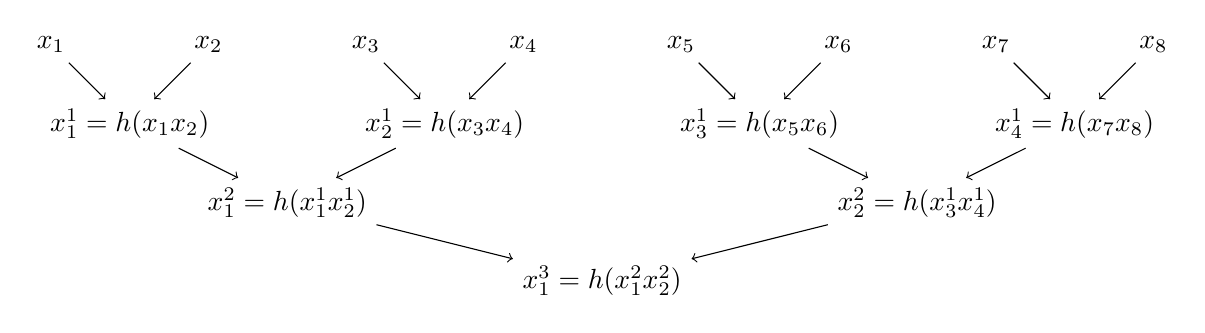
\begin{tikzpicture}[edge from parent/.style={draw,<-}, grow'=up]
\node{\(x^3_1=h(x^2_1x^2_2)\)} [level distance=10mm,sibling distance=80mm]
child { node{\(x^2_1=h(x^1_1x^1_2)\)} [level distance=10mm ,sibling distance=40mm]
  child {node {\(x^1_1=h(x_1x_2)\)}[level distance=10mm ,sibling distance=20mm]
    child {node {\(x_1\)}}
    child {node {\(x_2\)}}
  }
  child {node {\(x^1_2=h(x_3x_4)\)}[level distance=10mm ,sibling distance=20mm]
    child {node {\(x_3\)}}
    child {node {\(x_4\)}}}
}
child { node{\(x^2_2=h(x^1_3x^1_4)\)} [level distance=10mm ,sibling distance=40mm]
  child {node {\(x^1_3=h(x_5x_6)\)} [level distance=10mm ,sibling distance=20mm]
    child {node {\(x_5\)}}
    child {node {\(x_6\)}}
  }
  child {node {\(x^1_4=h(x_7x_8)\)}[level distance=10mm ,sibling distance=20mm]
    child {node {\(x_7\)}}
    child {node {\(x_8\)}}}
};
\end{tikzpicture}
\end{center}

Note that hashing with this kind of a tree is as strong as only applying \(h\) once, as we can see that a collision for the whole tree implies a collision somewhere within the tree.\smallskip

This is because two different inputs to the tree must necessarily result in different trees. But if they cause a collision, this means that there is some first level \(0<k\le m\) (going from top\(=0\) to bottom\(=m\)) where the two trees are exactly the same. This means that between levels \(k\) and \(k-1\), there was a collision somewhere. So anything that can produce a collision in the larger tree must necessarily produce a collision for the individual hash function.

\subsubsection{``Refreshing" the keys}
The idea propsed by Naor and Yung is a simple one, and it essentially involves chaining multiple keys together using a linked-list mechanism. \medskip

With hashing in mind, we create a first public key of length \(2n\), which is twice the length that we would need due to our hashing family. Then, we may sign a document using the first half of this key.\smallskip

The second half of the key will be reserved for signing a new key, which will be hashed down and then signed. We can continue this indefinitely, but note that by this mechanism, we aren't doing a whole lot better than before, since each key is only generating one new key, so we have linear growth.\medskip

If, instead, we used each key to sign two new keys (i.e., used both the first and second halves to sign different keys), then we would have exponential growth in the number of keys we have verified for our own use, which puts us in a much better spot. This is the mechanism/scheme that Naor and Yung proposed.

Note that with all this in mind, we may use a PRF to generate all the keys in our tree, and then we may sign and validate them all using this scheme. This works because as we have previously shown, PRF's are just about as good as true randomness.

\end{document}